\section{Introduction}

Segment Anything Models (SAM) adapted for 3D medical imaging~\citep{wang2023sam_med3d,du2023segvol,ma2024medsam,zhu2024medsam2} enable interactive organ segmentation through point prompts: a clinician clicks on a target organ, and the model produces a volumetric segmentation mask. This paradigm assumes a fundamental contract---changing the prompt target should change the predicted mask. The promise of such models lies precisely in this interactive controllability, which enables efficient annotation workflows and intraoperative guidance.

We discover that this contract is systematically violated. When evaluated on multi-organ abdominal CT, SAM-Med3D~\citep{wang2023sam_med3d} achieves only 20.8\% \emph{Switch Accuracy}---the rate at which the model correctly changes its prediction when the prompt moves from one organ to another (Figure~\ref{fig:problem}). The model predicts the same dominant organ regardless of prompt location, effectively ignoring user input. This means that in nearly 80\% of cases, clicking on a different organ produces the same segmentation output---a catastrophic failure for interactive clinical use.

\begin{figure*}[t]
\centering
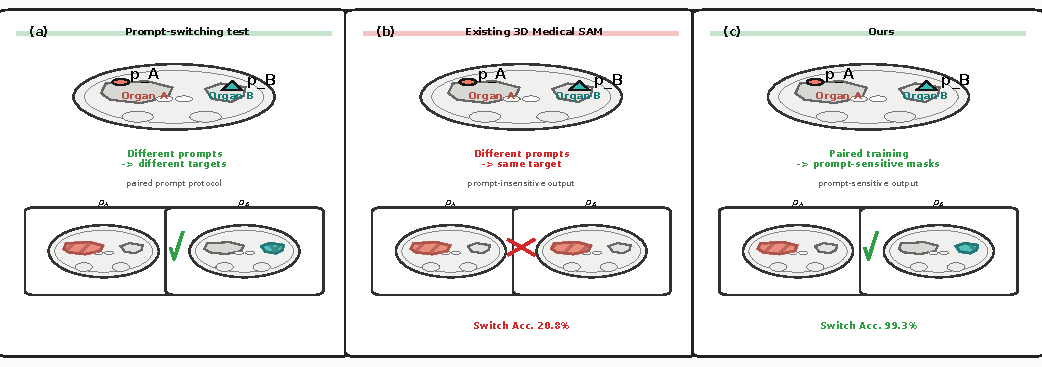
\includegraphics[width=0.95\textwidth]{figures/fig1_problem_overview.pdf}
\caption{Prompt unfaithfulness in 3D medical SAM. (a) Expected behavior: different point prompts should produce different segmentation masks. (b) Observed behavior: SAM-Med3D produces nearly identical predictions regardless of prompt target (Switch Accuracy = 20.8\%). (c) After our Paired Prompt-Contrastive Training: the model correctly switches predictions to match the prompted organ (Switch Accuracy = 99.3\%).}
\label{fig:problem}
\end{figure*}

This failure is \emph{not} a robustness problem. Recent work~\citep{chattopadhyay2026robustness} studies sensitivity to prompt perturbations, finding that models degrade under noise. In contrast, SAM-Med3D is remarkably robust to prompt noise (only 1.3-point Dice drop at 10-voxel perturbation). The failure we identify is a \emph{controllability} problem: the model has learned strong anatomical priors that override prompt information entirely. Standard Dice evaluation completely hides this problem because Dice rewards accurate segmentation regardless of whether the model actually follows the prompt.

We trace the root cause to single-prompt training. When each training step presents only one prompt per image, the model can achieve low segmentation loss by exploiting image priors---always predicting the largest or most salient organ---without learning prompt-conditioned behavior. The model never needs to demonstrate that different prompts produce different outputs. This is analogous to a language model that produces the same response regardless of the input query: technically functional but fundamentally uncontrollable.

Our fix is conceptually simple: \emph{Paired Prompt-Contrastive Training}. For each training image, we sample two organ prompts, compute predictions for both using a shared decoder, and supervise both outputs. This forces the model to produce different masks for different prompts on the same image---it can no longer satisfy the training objective by ignoring prompts. Through comprehensive mechanism ablation, we discover that this paired exposure is the dominant factor---achieving +40 points Switch Accuracy improvement---while auxiliary losses (grounding regularization, switch margin) provide only marginal additional benefit (+0--5 points).

Our contributions are:
\begin{enumerate}
    \item We identify \emph{prompt unfaithfulness} as a distinct failure mode in 3D medical SAM models, measurable via Switch Accuracy, and show it is hidden by standard Dice evaluation yet catastrophic for interactive use.
    \item We propose Paired Prompt-Contrastive Training and demonstrate through factor-isolation ablation that paired prompt exposure---not any specific loss function---is the core mechanism restoring faithfulness.
    \item We validate across datasets (AMOS, BTCV) with 3-seed experiments, achieving Switch Accuracy 0.993$\pm$0.012 with Dice 0.676$\pm$0.006, at only 5.3\% training overhead and zero inference cost.
    \item We show that prompt unfaithfulness is specific to 3D medical SAM adaptation (SAM2 achieves 0.954 Switch on natural images), suggesting it arises from limited medical training data and strong anatomical priors.
\end{enumerate}
